\section{Appendix: Process to Date}
With respect to the presented timeline (Table~\ref{table:timeline}) in Section.~\ref{timeline}, this section provides a brief review of the process to date of the PhD thesis work. The works focused on the objectives of: wildfire image restoration, wildfire detection, and fire fronts prediction. They are separately stated as follow.
\subsection{Wildfire Image Restoration}
To develop the robustness of GAN for wildfire image restoration, a feature loss is proposed to improve the original confusion loss of U-net-based GAN. The simulation programmings of the restoration are illustrated in Table~\ref{table:GANprogram}.
\begin{table}[ht]
\caption{The simulation basement of proposed feature loss GAN for wildfire image restoration}
\label{table:GANprogram}
    \centering
    \small
    \begin{tabular}{c c}
    \toprule
        Names & Illustrations\\
        \hline
        \rowcolor{mygray}
        Platform & Google Cloud Platform (GCP)\\
        Framework &  Pytorch, Fastai\\
        \rowcolor{mygray}
        GPU & nvidia-tesla-t4\\
        GAN Structure & ResNet-based U-net\\
        \rowcolor{mygray}
        Feature Loss Network& VGG16-based U-net\\
        Dataset Resource& Google Images \\
    \bottomrule
    \end{tabular}
\end{table}\par
The training process losses are shown in Fig.~\ref{fig:GANlosscompare}. There is an obvious jumping of validation loss as the entire U-net structure of GAN is unfreezed, which shows the jumping out of local minimum.
\begin{figure}[ht]
\centering
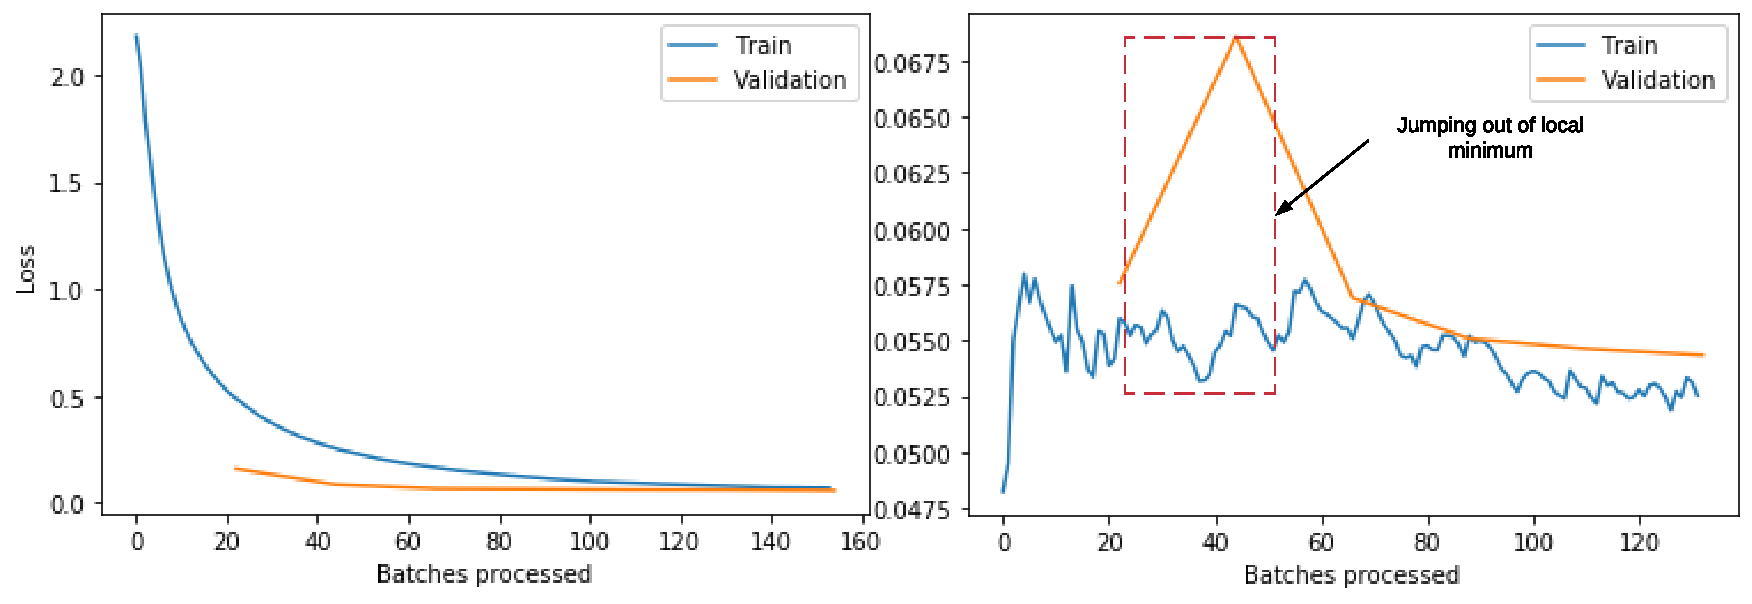
\includegraphics[height=50mm]{figs/GANlosscompare.pdf}
\caption{U-net training loss and validation loss changing. Left: Freeze encoder part of U-net; Right: Unfreezed encoder-decoder U-net. It seems over trained but jumped out of local minimum.}
\label{fig:GANlosscompare}
\end{figure}\par
 The final restoration performance is shown in Fig.~\ref{fig:GANoutcompare} by comparing with the single VGG16-based GAN, the proposed model shows higher robustness.
\begin{figure}[ht]
\centering
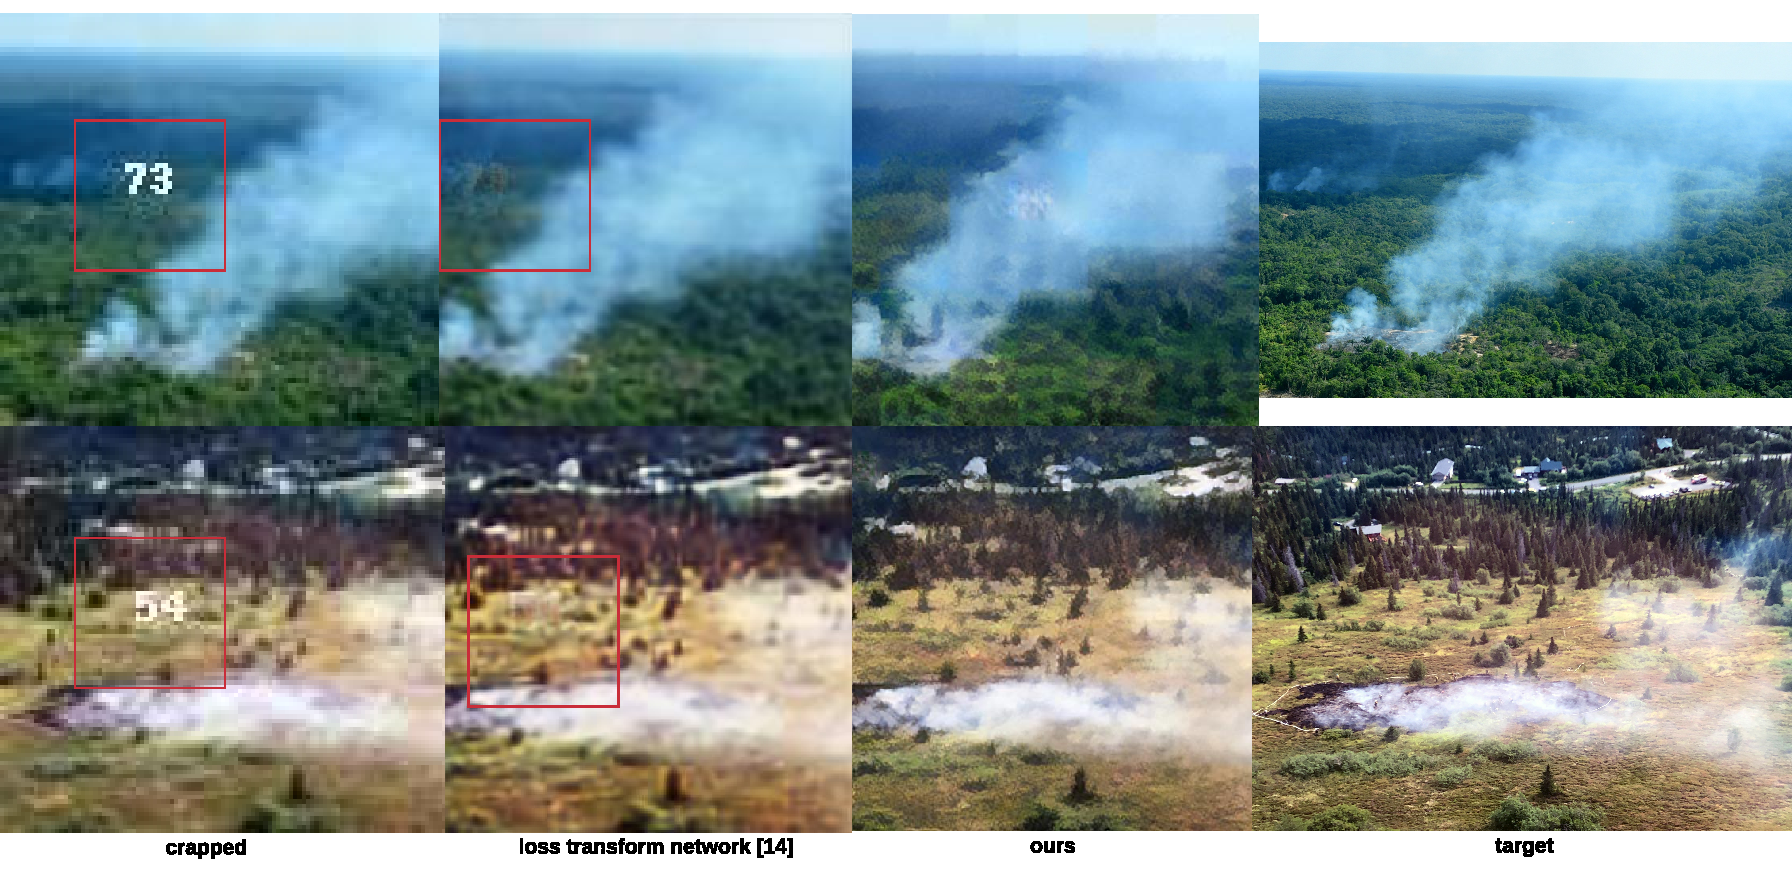
\includegraphics[height=60mm]{figs/GANoutcompare.pdf}
\caption{The GAN restoration output. Left column: Crapped images, number marks are randomly added as disturbance at random location in images, higher number order means the image is randomly crapped more. Mid-left column: Restoration results of feature loss network. Mid-right column: Restoration results of proposed loss GAN. Right column: Original images (targets).}
\label{fig:GANoutcompare}
\end{figure}\par

\subsection{Wildfire Classification}
The wildfire images classification is designed for UAV or UAVs to discriminate whether there suspected smoke or flame is contained in the image. This program is working before the segmentation on-board. Because the segmentation program might cause more computation and energy cost of on-board computer and battery. The designed classification contains ResNet34 based classifier and developed attention mechanism-based classifier. Their simulation basement are stated in Table.~\ref{table:classprogram}, and their classification results are shown as follow in Fig.~\ref{fig:classresnetattention}.
\begin{table}[ht]
\centering
\caption{The simulation basement of proposed ResNet34-based and Attention mechanism-based wildfire classifiers}
\label{table:classprogram}
    \small
    \begin{tabular}{c c c}
    \toprule
        Names & ResNet34-based Classifier &  Attention-based Classifier\\
        \hline
        Dataset Source& \multicolumn{2}{c}{Google Images, Kaggle Dataset}\\
        \rowcolor{mygray}
        Platform & \multicolumn{2}{c}{
        Personal Computer}\\
        Framework &  \multicolumn{2}{c}{Pytorch, Fastai}\\
        \rowcolor{mygray}
        CPU & \multicolumn{2}{c}{Intel-i7-4790K}\\
        \rowcolor{mygray}
        GPU & Nvidia-GTX-1060 & Nvidia-GTX-1660\\
        Pre-Training & False & ImageNet\\
    \bottomrule
    \end{tabular}
\end{table}
\begin{figure}[ht]
\centering
    \begin{subfigure}{.3\linewidth}
    \centering
        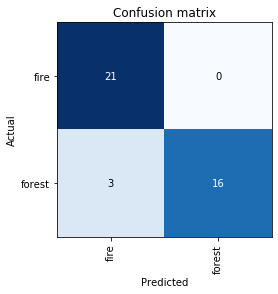
\includegraphics[width=50mm]{figs/classrensnet.png}
        \caption{}
    \end{subfigure}
    \begin{subfigure}{.3\linewidth}
    \centering
        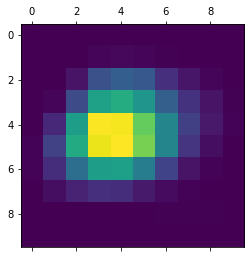
\includegraphics[width=50mm]{figs/classattention.png}
        \caption{}
    \end{subfigure}
    \begin{subfigure}{.3\linewidth}
    \centering
        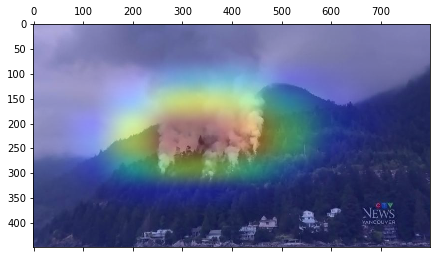
\includegraphics[width=50mm,height=50mm]{figs/classattention2.png}
        \caption{}
    \end{subfigure}
    \caption{\small Classification results of designed classifiers. (a) The confusion matrix of ResNet34-based wildfire classification. (b) The result heat-map of Attention-based wildfire classification. (c) The mixed heat-map mask and original image.}
    \label{fig:classresnetattention}
\end{figure}\par

\subsection{Wildfire Segmentation}
When the image is demonstrated as a wildfire image, it will be send into the segmentation program part so that the wildfire detection accuracy could be increased and the suspected fire point could be located more specific in the image.\par
The designed segmentation model on-board is based on pure U-net which has ResNet18 structure and the H20T infrared camera could be applied for directly detect the wildfire with appropriate threshold. The segmentation model on ground work station is based on ResNet34. For both the model on-board and on ground work station, attention mechanism and squeezed model should be designed to develop the model. The simulation and experience basement are separately illustrated in Table~\ref{table:segprogram}.
\begin{table}[ht]
\centering
\caption{The simulation basement of proposed on-board and ground segmentation model}
\label{table:segprogram}
    \small
    \begin{tabular}{c c c}
    \toprule
        Names & On-board Segmentation Model & Ground Segmentation Model\\
        \hline
        Dataset Source& \multicolumn{2}{c}{Kaggle Dataset, UAV Captured Experience Dataset}\\
        \rowcolor{mygray}
        Platform & YunGuan on-board computer with DJI M300 UAV& Personal Computer\\
        Framework &  DJI OSDK, ROS, Pytorch & Pytorch, Fastai\\
        \rowcolor{mygray}
        CPU & NAN& {Intel-i7-4790K}\\
        \rowcolor{mygray}
        GPU & Nvidia-Jetson & Nvidia-GTX-1660\\
        \rowcolor{mygray}
        Model Structure& ResNet18& ResNet34\\
        Pre-Training & ImageNet & ImageNet\\
    \bottomrule
    \end{tabular}
\end{table}
\par
As shown in Fig.~\ref{fig:segmentationGround} is the segmentation results of the proposed ResNet34-based U-net with attention gates in skip connection. The targets are frames randomly from a video captured by UAV, which is the dataset from Kaggle. The right column shows that the original designed model is sensitive, but with higher false positive. The developed model with attention gate sacrificed the sensitivity but decreased the false positive and increased accuracy.
\begin{figure}[ht]
    \centering
    \begin{subfigure}{.24\linewidth}
    \centering
        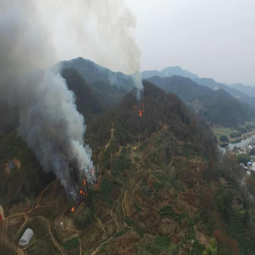
\includegraphics[width = 38mm]{figs/ain1.png}
    \end{subfigure}
    \begin{subfigure}{.24\linewidth}
    \centering
        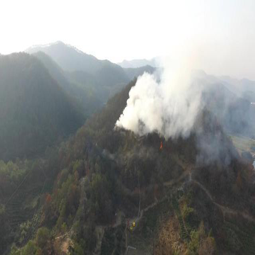
\includegraphics[width = 38mm]{figs/ain2.png}
    \end{subfigure}
        \begin{subfigure}{.24\linewidth}
    \centering
        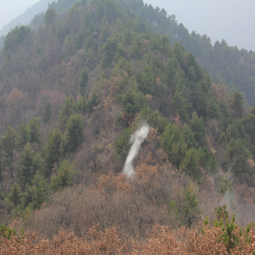
\includegraphics[width = 38mm]{figs/ain3.png}
    \end{subfigure}
    \begin{subfigure}{.24\linewidth}
    \centering
        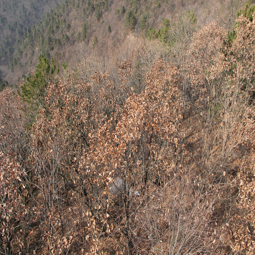
\includegraphics[width = 38mm]{figs/ain4.png}
    \end{subfigure}
        \begin{subfigure}{.24\linewidth}
    \centering
        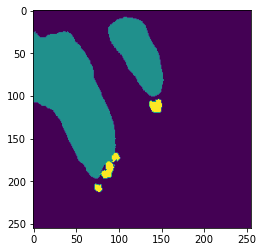
\includegraphics[width = 41mm]{figs/aunet1.png}
    \end{subfigure}
    \begin{subfigure}{.24\linewidth}
    \centering
        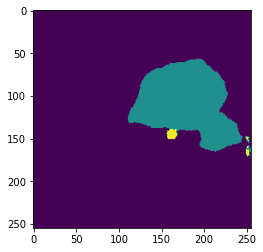
\includegraphics[width = 41mm]{figs/aunet2.png}
    \end{subfigure}
        \begin{subfigure}{.24\linewidth}
    \centering
        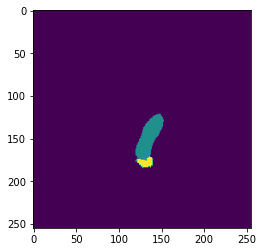
\includegraphics[width = 41mm]{figs/aunet3.png}
    \end{subfigure}
    \begin{subfigure}{.24\linewidth}
    \centering
        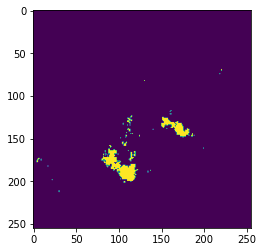
\includegraphics[width = 41mm]{figs/aunet4.png}
    \end{subfigure}
        \begin{subfigure}{.24\linewidth}
    \centering
        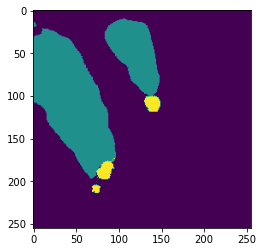
\includegraphics[width = 41mm]{figs/atunet1.png}
    \end{subfigure}
    \begin{subfigure}{.24\linewidth}
    \centering
        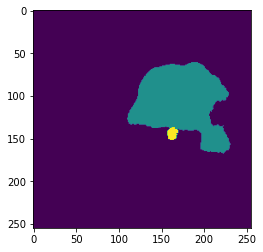
\includegraphics[width = 41mm]{figs/atunet2.png}
    \end{subfigure}
        \begin{subfigure}{.24\linewidth}
    \centering
        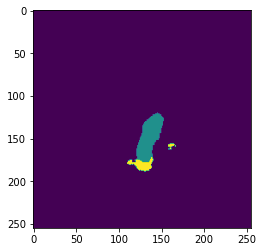
\includegraphics[width = 41mm]{figs/atunet3.png}
    \end{subfigure}
    \begin{subfigure}{.24\linewidth}
    \centering
        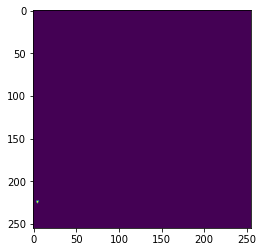
\includegraphics[width = 41mm]{figs/atunet4.png}
    \end{subfigure}
\caption{Segmentation results of ResNet34-based U-net on ground work station. Left two columns: Targets on Kaggle and segmentation results. Right two columns: Experience video data captured by DJI Phantom 4 UAV. Top row: Targets. Mid row: Segmentation results of the designed model. Bottom row: Segmentation results of the designed model developed by attention gates.}
\label{fig:segmentationGround}
\end{figure}\par
As shown in Fig.~\ref{fig:segmentationUAV} is the experience results of the on-board detection. The designed ResNet18 is successfully deployed on DJI M300 UAV. The experience demonstrated that the work of model size decreasing is acceptable. However, the model has not been developed yet. In the first time experience, accuracy is sacrificed to ensure the stable flight and decrease the detection as building the light model. At the start period of experience, the cloud is detected as smoke, which means the model still need more adjustment.
\begin{figure}[ht]
\centering
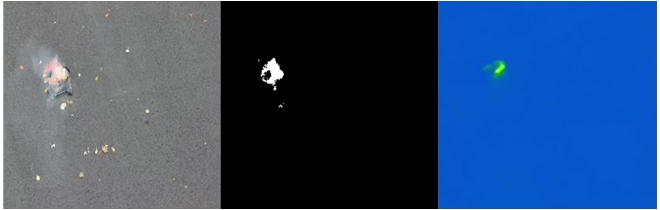
\includegraphics[height=40mm]{figs/test.jpg}
\caption{On-board segmentation result. Left: Masked original image. Mid: Segmentation mask. Right: infrared camera image.}
\label{fig:segmentationUAV}
\end{figure}\par
\subsection{Wildfire Prediction}
The wildfire prediction is based on Cellular model and developed through LSTM. The results could be illustrated in Fig.~\ref{fig:prediction}, it could be demonstrated that the wind impacts the wildfire spreading most heavily.
